\documentclass{ijsra}
\def\IJSRAidentifier{\currfilebase} %<---- don’t change this!
%-------Title | Email | Keywords | Abstract-------------
\def\shorttitle{Professor Chris Stringer}
\def\maintitle{Professor Chris Stringer, Ph.D.
\textit{Merit Researcher at the Natural History Museum, London, 
Visiting Professor at Royal Holloway and Honorary Professor at University College London}}
\def\cmail{hannah.ryan@arch.ox.ac.uk}
\def\keywords{Interview}
%\def\keywordname{}%<--- redefine the name “Keywords“ in needed language
\def\abstract{}
%--------Author’s names------------
\def\authorone{Hannah F. Ryan}
%-------Biographical information-------------
\def\bioone{PhD Student at the Research Laboratory in Archaeology and History of Art, University of Oxford, UK.}
%------University/Institution--------------
\def\affilone{Department of Archaeology and History of Art, University of Oxford, UK}
%--------Mapping of authors to affiliations------------
%% authorone:--> * <--- copy/paste that symbol to \affiloneauthor etc. below
%-------------------------------------------------------------------------
%\def\affiloneauthor{*}%<---- paste the symbol of the authors into {}

\begin{filecontents}{\IJSRAidentifier.bib}
%Bibliography-data HERE
\end{filecontents}
\begin{document}
\IJSRAopening
%-------

\begin{figure}[!htb] %FIGURE 1
	\centering
	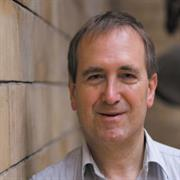
\includegraphics[width=\linewidth]{Stringer_Figure1}
	\caption{
	{\normalfont\scriptsize \copyright\ by
                 % or NAME OF COPYRIGHT HOLDER
                  }}
	\label{fig:Stringer_Figure1}
\end{figure}

\textbf{IJSRA (International Journal of Student Research in Archaeology)}: 
\textit{When and why did you become interested in physical anthropology?}
 
\textbf{CS (Prof. Chris Stringer)}: My interest in human evolution started at primary school.
I was fascinated by fossils, and at the age of nine or ten did a school project on Neanderthals – I wish I still had it!
My interest grew through my school years but I had no idea that you could actually study in this area, so I planned to do medicine.
I had a place at medical school lined up, when I chanced upon University College London’s prospectus.
It was arranged alphabetically, and Anthropology was at the beginning.
The course offered archaeology, human evolution, genetics and social anthropology.
Suddenly medicine seemed much less appealing.
So I phoned UCL (this was long before the internet!), was invited for an interview, and offered a place.
Much to the amazement of my teachers and parents, I dropped medicine and took up this study subject,
which I had only just learnt existed.
 
\textbf{IJSRA}: \textit{Do you think then that we need to publicise physical anthropology to younger audiences considering that you were
originally unaware that it was a subject area for study?}

\textbf{CS}: Well I was from a working-class background in the East End of London, looking at the career choices offered by
teachers and the school library in 1966. Today, with online resources and social media,
I think both those giving advice and those looking for options have so much more information – maybe too much, at times!

\textbf{IJSRA}: \textit{Your publications range in topic from morphology, dating, climate, primatology, and isotopes.
Do you enjoy the interdisciplinary nature of your work? 
Is specialism and collaboration the future for archaeology and anthropology or is being a generalist a viable career choice?}

\textbf{CS}: I do enjoy the breadth, but it’s increasingly difficult to be a generalist in our area because of
the pace of new developments in highly specialised fields like DNA and isotopes.
I have to spend a lot of time trying to keep up with just the latest on DNA and the evidence for ancient hybridisation – that’s only one (big and ever-growing) area. Choosing the right collaborators is crucial!

\textbf{IJSRA}: \textit{You’ve run projects on hominins at an international (RESET project) and a national scale (Pathways to Ancient Britain).
Which types of project do you think are most informative for physical anthropology?}

\textbf{CS}: I’ve been lucky enough to be involved in a few finds of new material (e.g. Gough’s Cave) but
those large projects which seek to significantly increase the fossil record are, of course,
some of the most important – think what has emerged from sites like Liang Bua (\textit{floresiensis}) and Rising Star (\textit{naledi})
in the last few years. 
There are so many gaps in the geographical and chronological coverage, even in Africa, let alone vast areas of Asia or Oceania!
But for me, it’s also important to revisit old collections and apply new techniques of investigation – things like direct dating,
isotopes, taphonomic studies. 
We did that very successfully with AHOB (Ancient Human Occupation of Britain) and now with PAB,
and a whole new area of aDNA has also opened up now, of course.

\textbf{IJSRA}: \textit{Currently you are a leading academic on research into hominins and you are often quoted when new discoveries
have emerged (such as the recent discovery of \textit{Homo naledi}). When you first started your research however,
your support for the ‘Recent African Origin’ (RAO) hypothesis was in the minority as most supported the multi regionalism model.
Was it a relief when the RAO theory gained more support?}

\textbf{CS}: Well when I finished my PhD in 1974 I was pretty sure that modern humans had not evolved from European Neanderthals but
it took another decade before I was more certain that we had an African origin.
However this still-minority view was not really taken seriously until breakthroughs in DNA and dating in the late
1980s – then the polarisation and conflict really started to take off!

\textbf{IJSRA}: \textit{Recent research on hominin DNA and the discovery of hybridization, has led to some academics reverting back to
the multiregional model. 
Others suggest that now the human origins answer falls somewhere between the two.
What has been your experience in accepting (or rejecting) new research that usurps well established theory?}

\textbf{CS}: I’ve certainly learnt to expect the unexpected in the last few years!
I’d refer your readers to my book \textit{The Origin of our Species (Lone Survivors in the USA)} for more on how my views have changed,
and sometimes been forced to change!
Because we are human beings, and often very much in the public and media eye, it’s sometimes hard to
admit that we might have got it wrong, but as scientists it’s our duty to do so!
Presenting clear and testable ideas is a valuable service to science, but only if those ideas are at least credible in the first place.

\textbf{IJSRA}: \textit{With ancient DNA techniques, researchers have found both hybridization behaviour as well as
previously undiscovered hominins.
In your opinion, do you think this will lead to an assumption of a more diverse and bushy hominin phylogeny or
a more refined hominin family tree (lumping vs splitting classification)?}

\textbf{CS}: I think a bushy tree is already a reality but the species question applied to fossils is always going to be problematic.
I still think on morphology that the Neanderthals are specifically distinct from everyone alive today – they can be
distinguished just from their ear bones, for example.
But accepting that doesn’t mean accepting that they were reproductively isolated from us, as they clearly were not.
Closely-related mammal and bird species may take millions of years to become fully isolated from each other genetically.

\textbf{IJSRA}: \textit{You are currently affiliated with both the Natural History Museum and multiple Universities.
In your experience what are the main differences and advantages to working in these types of institutions?}

\textbf{CS}: I’ve got visiting/honorary professorships at two London Universities, so can make some comparisons.
A Museum can be a highly bureaucratic place at times, but it also has wonderful collections - and staff.
Having students around can be a great stimulus, but supervisions and assessments can take up a lot of time!
But I wouldn’t be where I am without some inspirational teaching and supervision along the way – and
I would take that comment right back to my primary schools!

\textbf{IJSRA}: \textit{As an academic who works in a museum, do you feel that current research reaches the general public?}

\textbf{CS}: I’ve always been aware of the need for outreach and have enjoyed contributing in the media and
giving talks to general audiences.
I do feel it is our responsibility to communicate beyond a purely academic audience, and I feel that an increasing number of
my colleagues share that view. 
Of course not everyone is a great communicator, but we can all try and do our bit!

\textbf{IJSRA}: \textit{Research on hominins generates a lot of media attention.
What are the benefits and draw backs of this interest and do you have a strategy for working with media outlets?}

\textbf{CS}: When there is a big story, it can take over your life for a few days if you let it,
and you always have to judge if it’s worth the time against the other things you were hoping to do!
Some stories are undoubtedly over-hyped or even completely misguided and I try to avoid engaging with those.
Our NHM press team is great at helping me manage the media storms which sometimes arise!

\textbf{IJSRA}: \textit{Our journal attempts to give a platform for archaeology students to publish in the early stages of their research.
Are open platforms and publications a valuable resource?}

\textbf{CS}: I do think open platforms and publications are valuable – my open access publication on \textit{Homo naledi} has
very quickly overtaken most of my other publications in terms of impact.
Undergrads need to get their formative ideas out there but they must also be prepared for the critiques
(some more measured and warranted than others) that almost always follow open access publication!

\textbf{IJSRA}: \textit{If you could go back to your undergraduate self, what piece of advice would you give?
Would you give this same advice to undergraduates now?}

\textbf{CS}: I think both then and now it’s to have a plan A and a plan B for your future.
I’ve been lucky enough that plan A has usually worked out, but putting all your eggs in one basket is not a good idea!
Also network as much as you can and try not to make enemies – you never know who you might need help from in the future!

Professor Chris Stringer is currently a merit researcher at the Natural History Museum but also holds
an honorary professorship at University College London and is a visiting professor at Royal Holloway.
He is a fellow of the American Association for the Advancement of Science, Washington and the Royal Society as well as
being an Honorary fellow of the Society of Antiquities. 
He won the River’s Memorial Medal (2004) from the Royal Anthropological Institute and the Frink medal (2008) from
the Zoological Society of London. His early career was on the role of Neanderthals in hominin history,
leading to his role in the development of the Recent African Origin theory.
He now collaborates with a range of academics on projects intended to improve our understanding of hominin evolution.
Professor Stringer first studied Anthropology at University College London followed by a PhD at Bristol in Anatomical Science.
He has published papers in their hundreds and several books, one of the most recent being \textit{The Origin of Our Species},
published in the United States as \textit{Lone Survivors: How We Came to Be the Only Humans on Earth}.

\IJSRAclosing
\end{document}
